\documentclass[12pt, spanish]{article}
\usepackage[spanish]{babel}
\selectlanguage{spanish}
%\usepackage{natbib}
\usepackage{url}
\usepackage[utf8x]{inputenc}
\usepackage{graphicx}
\graphicspath{{images/}}
\usepackage{parskip}
\usepackage{fancyhdr}
\usepackage{vmargin}
\usepackage{multirow}
\usepackage{float}
\usepackage{chngpage}
\usepackage{enumitem}
\usepackage{forloop}


\usepackage{amsfonts}

\usepackage{subcaption}

\usepackage{hyperref}
\usepackage[
    type={CC},
    modifier={by-nc-sa},
    version={4.0},
]{doclicense}

\hypersetup{
    colorlinks=true,
    linkcolor=blue,
    filecolor=magenta,
    urlcolor=cyan,
}

% para codigo
\usepackage{listings}
\usepackage{xcolor}



%% configuración de listings

\definecolor{listing-background}{HTML}{F7F7F7}
\definecolor{listing-rule}{HTML}{B3B2B3}
\definecolor{listing-numbers}{HTML}{B3B2B3}
\definecolor{listing-text-color}{HTML}{000000}
\definecolor{listing-keyword}{HTML}{435489}
\definecolor{listing-identifier}{HTML}{435489}
\definecolor{listing-string}{HTML}{00999A}
\definecolor{listing-comment}{HTML}{8E8E8E}
\definecolor{listing-javadoc-comment}{HTML}{006CA9}

\lstdefinestyle{eisvogel_listing_style}{
  language         = python,
%$if(listings-disable-line-numbers)$
%  xleftmargin      = 0.6em,
%  framexleftmargin = 0.4em,
%$else$
  numbers          = left,
  xleftmargin      = 0em,
 framexleftmargin = 0em,
%$endif$
  backgroundcolor  = \color{listing-background},
  basicstyle       = \color{listing-text-color}\small\ttfamily{}\linespread{1.15}, % print whole listing small
  breaklines       = true,
  frame            = single,
  framesep         = 0.19em,
  rulecolor        = \color{listing-rule},
  frameround       = ffff,
  tabsize          = 4,
  numberstyle      = \color{listing-numbers},
  aboveskip        = 1.0em,
  belowskip        = 0.1em,
  abovecaptionskip = 0em,
  belowcaptionskip = 1.0em,
  keywordstyle     = \color{listing-keyword}\bfseries,
  classoffset      = 0,
  sensitive        = true,
  identifierstyle  = \color{listing-identifier},
  commentstyle     = \color{listing-comment},
  morecomment      = [s][\color{listing-javadoc-comment}]{/**}{*/},
  stringstyle      = \color{listing-string},
  showstringspaces = false,
  escapeinside     = {/*@}{@*/}, % Allow LaTeX inside these special comments
  literate         =
  {á}{{\'a}}1 {é}{{\'e}}1 {í}{{\'i}}1 {ó}{{\'o}}1 {ú}{{\'u}}1
  {Á}{{\'A}}1 {É}{{\'E}}1 {Í}{{\'I}}1 {Ó}{{\'O}}1 {Ú}{{\'U}}1
  {à}{{\`a}}1 {è}{{\'e}}1 {ì}{{\`i}}1 {ò}{{\`o}}1 {ù}{{\`u}}1
  {À}{{\`A}}1 {È}{{\'E}}1 {Ì}{{\`I}}1 {Ò}{{\`O}}1 {Ù}{{\`U}}1
  {ä}{{\"a}}1 {ë}{{\"e}}1 {ï}{{\"i}}1 {ö}{{\"o}}1 {ü}{{\"u}}1
  {Ä}{{\"A}}1 {Ë}{{\"E}}1 {Ï}{{\"I}}1 {Ö}{{\"O}}1 {Ü}{{\"U}}1
  {â}{{\^a}}1 {ê}{{\^e}}1 {î}{{\^i}}1 {ô}{{\^o}}1 {û}{{\^u}}1
  {Â}{{\^A}}1 {Ê}{{\^E}}1 {Î}{{\^I}}1 {Ô}{{\^O}}1 {Û}{{\^U}}1
  {œ}{{\oe}}1 {Œ}{{\OE}}1 {æ}{{\ae}}1 {Æ}{{\AE}}1 {ß}{{\ss}}1
  {ç}{{\c c}}1 {Ç}{{\c C}}1 {ø}{{\o}}1 {å}{{\r a}}1 {Å}{{\r A}}1
  {€}{{\EUR}}1 {£}{{\pounds}}1 {«}{{\guillemotleft}}1
  {»}{{\guillemotright}}1 {ñ}{{\~n}}1 {Ñ}{{\~N}}1 {¿}{{?`}}1
  {…}{{\ldots}}1 {≥}{{>=}}1 {≤}{{<=}}1 {„}{{\glqq}}1 {“}{{\grqq}}1
  {”}{{''}}1
}
\lstset{style=eisvogel_listing_style}


\usepackage[default]{sourcesanspro}

\setmarginsrb{2 cm}{1 cm}{2 cm}{2 cm}{1 cm}{1.5 cm}{1 cm}{1.5 cm}

\title{Práctica 4:\\
Modelos de Simulación Dinámicos Continuos.\hspace{0.05cm} }
\author{Antonio David Villegas Yeguas}
\date{\today}

\renewcommand*\contentsname{hola}

\makeatletter
\let\thetitle\@title
\let\theauthor\@author
\let\thedate\@date
\makeatother

\pagestyle{fancy}
\fancyhf{}
\rhead{\theauthor}
\lhead{\thetitle}
\cfoot{\thepage}

\begin{document}

%%%%%%%%%%%%%%%%%%%%%%%%%%%%%%%%%%%%%%%%%%%%%%%%%%%%%%%%%%%%%%%%%%%%%%%%%%%%%%%%%%%%%%%%%

\begin{titlepage}
    \centering
    \vspace*{0.3 cm}
    
\includegraphics[scale = 0.50]{ugr.png}\\[0.7 cm]
    %\textsc{\LARGE Universidad de Granada}\\[2.0 cm]
    \textsc{\large 4º CSI 2020/21 - Grupo 1}\\[0.5 cm]
    \textsc{\large Grado en Ingeniería Informática}\\[0.5 cm]
    \rule{\linewidth}{0.2 mm} \\[0.2 cm]
    { \huge \bfseries \thetitle}\\
    \rule{\linewidth}{0.2 mm} \\[1 cm]

    \begin{minipage}{0.4\textwidth}
        \begin{flushleft} \large
            \emph{Autor:}\\
            \theauthor\\
			 \emph{DNI:}\\
            77021623-M
            \end{flushleft}
            \end{minipage}~
            \begin{minipage}{0.4\textwidth}
            \begin{flushright} \large
            \emph{Asignatura: \\
            Simulación de Sistemas}   \\
            \emph{Correo:}\\
            advy99@correo.ugr.es
        \end{flushright}
    \end{minipage}\\[0.5cm]

    {\large \thedate}\\[0.5cm]
    %{\url{https://github.com/advy99/AA/}}
    {\doclicenseThis}

    \vfill

\end{titlepage}

%%%%%%%%%%%%%%%%%%%%%%%%%%%%%%%%%%%%%%%%%%%%%%%%%%%%%%%%%%%%%%%%%%%%%%%%%%%%%%%%%%%%%%%%%

\tableofcontents
\pagebreak

%%%%%%%%%%%%%%%%%%%%%%%%%%%%%%%%%%%%%%%%%%%%%%%%%%%%%%%%%%%%%%%%%%%%%%%%%%%%%%%%%%%%%%%%%


\section*{Introducción}

En esta práctica estudiaremos un modelo de proparación de una enfermedad infecciosa, denominado modelo SIR.

Este modelo tendrá una población de cierto número de individuos, y podemos dividir los individuos en tres grupos:

\begin{enumerate}
	\item Supceptibles (S): No tienen la enfermedad, pero pueden contraerla.
	\item Infectados (I): Tienen la enfermedad y pueden contagiarla.
	\item Retirados (R): Han superado la enfermedad, no la contagian y no pueden volver a infectarse ya que o se han hecho inmunes o han muerto.
\end{enumerate}

Para esta práctica también haremos las siguientes suposiciones:

\begin{itemize}
	\item La población se mantiene constante, no se tienen en cuenta los nacimientos y muertes que se producen durante la simulación.
	\item La enfermedad no tiene periodo de incubación y se transmite por contacto directo. Si un individuo se infecta pasa del grupo S al grupo I automaticamente.
	\item La inmunidad es permanente, cuando un individuo pasa del grupo I al R ya no puede volver contraer la enfermedad.
	\item La tasa de infección depende del número de contactos entre individuos, es proporcional a $S(t) * I(t)$.
	\item Los individuos infectados mantendrán la enfermedad durante un periodo de tiempo determinado proporcional a $I(t)$.
\end{itemize}

Como nos comenta el guión, todas estas condiciones nos generan un sistema de tres ecuaciones diferenciales no lineales. El objetivo de esta práctica será simular este sistema partiendo de unas condiciones iniciales $S_0$, $I_0$ y $R_0$ que representen el valor inicial de individuos supceptibles, infectados y recuperados.

\section{Creación del modelo de simulación para el sistema}

Para la implementación del sistema he utilizado C++ basandome en el pseudocódigo dado. He decidido encapsular el modelo en una clase de C++ ya que muchos parámetros se conocen entre si y las funciones a implementar forman parte del modelo, además de que esta encapsulación nos permite una forma facil de modificar y adaptar el modelo a nuevas versiones más complejas y detalladas manteniendo su uso.

El modelo tendrá un constructor al que se le pasarán los parámetros necesarios, así como una implementación del operador de entrada que nos permitirá leer los parámetros desde fichero, entrada estandar o cualquier otro flujo de datos.


Una vez realizada la entrada de datos, el modelo tendrá un único método publico \texttt{simular}, con el que comenzaremos la simulación con los parámetros dados. Esta simulación simplemente modificará el estado actual del sistema (las variables I, S y R) mientras que el tiempo de simulación sea menor al tiempo de fin. Esta actualización del estado se podrá hacer tanto por el método de Runge Kutta como por el método de Euler. La implementación de estos métodos es como la dada en el pseudocódigo.

\section{Pruebas del sistema}

De cara a realizar las distintas pruebas del sistema utilizaremos el método de integración de Runge-Kutta con un intervalo de cálculo de $0.1$, a excepción de la comparación enter el método de Euler y el método de Runge-Kutta donde compararemos ambos métodos con distintos valores para el intervalo de cálculo.

\subsection{Prueba básica de funcionamiento}

Para comprobar el funcionamiento del sistema he lanzado la simulación como nos dice en el enunciado, con los parámetros $a = 0.001$ y $b = 0.125$, obteniendo los siguientes resultados:

\begin{figure}[H]
  \centering
      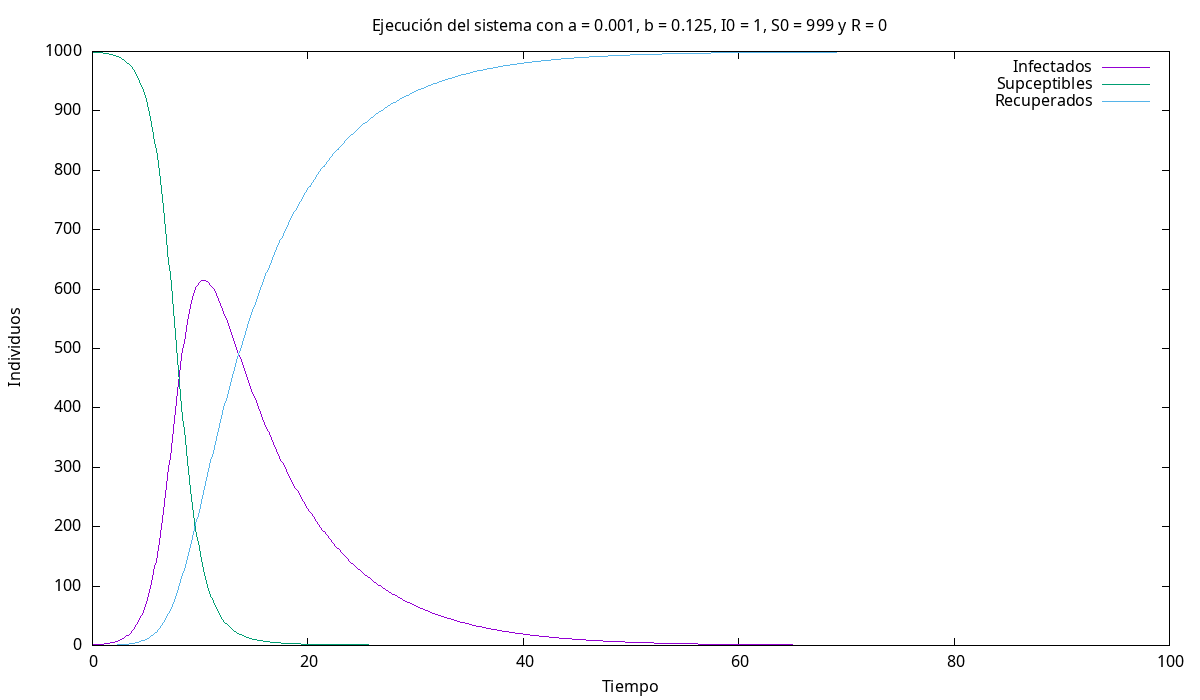
\includegraphics[width=\textwidth]{SIR_prueba_basica.png}
 		\caption{Prueba inicial del sistema.}
\end{figure}

Como vemos, el sistema funciona como esperabamos, al inicio con un único infectado y mucha población supceptible la curva de infectados crece de forma exponencial, sin embargo, la población al ser constante llega un punto en que la población supceptible es mucho menor ya que la mayoría ya están infectados o recuperados, por lo que la curva de infectados decae, hasta llegar a cero, momento en el que toda la población ha pasado la enfermedad y se ha recuperado.

\subsection{Modificaciones de individuos supceptibles iniciales en función de b/a}

Como se nos comenta en el guión, la constante $a$ está relacionada con la capacidad de infección de la enfermedad, mientras que $b$ está relacionada con el tiempo que dura la infección, en concreto, si la enfermedad dura $d$ días, $b = 1/d$ (para el apartado anterior, la enfermedad dura ocho días).

De forma que lo que nos pide en concreto este apartado es comprobar la relación que existe entre el tiempo que dura la infección con la capacidad de infección de la enfermedad.

Para realizar este apartado he mantenido el número de invididuos de la prueba inicial, y modificaré los valores de $a$ y $b$.

\subsubsection{Individuos supceptibles iniciales menor que b/a}

En este apartado concreto, si tenemos un número de individuos supceptibles menor que $b/a$ queremos que $1000 < b/a$, de forma que si mantenemos $a$ constante a $0.001$ tenemos que $b > 1$, y como $b = 1/d$, la duración de la enfermedad, $d$ ha de ser muy baja. Para la prueba usaré $b = 1.1$, de forma que $S_0 = 999 < 1.1/0.001$.

\begin{figure}[H]
  \centering
      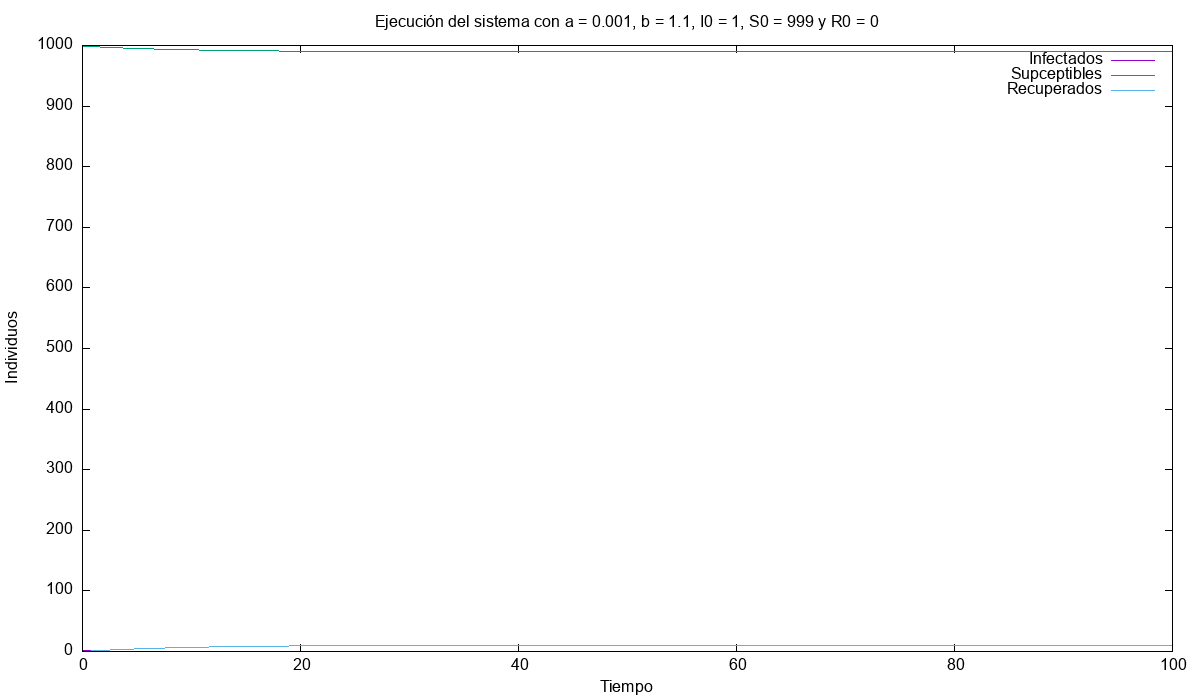
\includegraphics[width=\textwidth]{SIR_s0_menor.png}
 		\caption{Prueba del sistema con $S_0 < b/a$.}
\end{figure}

Observamos como el haber obligado a que la duración de la enfermedad sea tan baja hace que el tiempo en la que se puede propagar por la población están bajo, que los infectados se recuperan antes de infectar a la población supceptible, haciendo que la enfermedad desaparezca por no expandirse.

\subsubsection{Individuos supceptibles iniciales mayor que b/a}

En este apartado, si tenemos un número de individuos supceptibles mayor que $b/a$ queremos que $1000 > b/a$, de forma que si mantenemos $a$ constante a $0.001$ tenemos que $b < 1$, y como $b = 1/d$, la duración de la enfermedad, $d$ ha de ser más alta. Este caso es el caso de la prueba inicial que hemos realizado, donde $b$ era mucho menor que uno, y al tener una duración de enfermedad más alta y manteniendo $a$, la constante asociada a la tasa de infección, es de esperar que se infecte un número mucho mayor de la población. Para esta prueba, aunque nos vale con el apartado inicial, por probar con otros valores he probado con $b = 0.5$, es decir, la duración de la enfermedad será de dos días:

\begin{figure}[H]
  \centering
      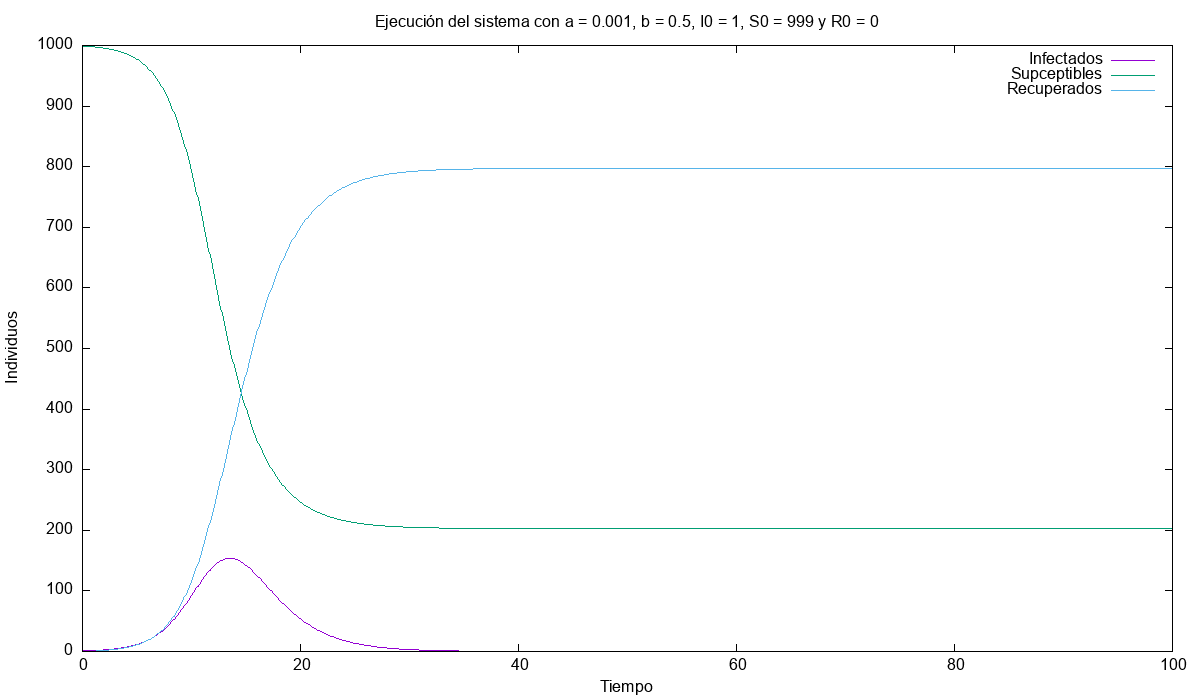
\includegraphics[width=\textwidth]{SIR_s0_mayor.png}
 		\caption{Prueba del sistema con $S_0 > b/a$.}
\end{figure}

Vemos como en este caso si se llega a infectar una mayor parte de la población, ya que tiene un periodo de dos días para infectar, sin embargo no llegamos a infectar a la población completa como en la primera prueba, ya que esta tenia un periodo de enfermedad de 8 días, cuatro veces el que hemos introducido en este ejemplo. Aun así, como comparación podemos concluir que esta relación entre $a$ y $b$ es muy importante de cara a la capacidad de infección de una persona y el tiempo que puede infectar, ya que es la que permite a la enfermedad propagarse.




\section{Evolución del sistema}

De cara a observar la evolución del sistema también vamos a graficar el avance de los recuperados respecto al plano de supceptibles e infectados utilizando los resultados de la prueba inicial:


\begin{figure}[H]
  \centering
      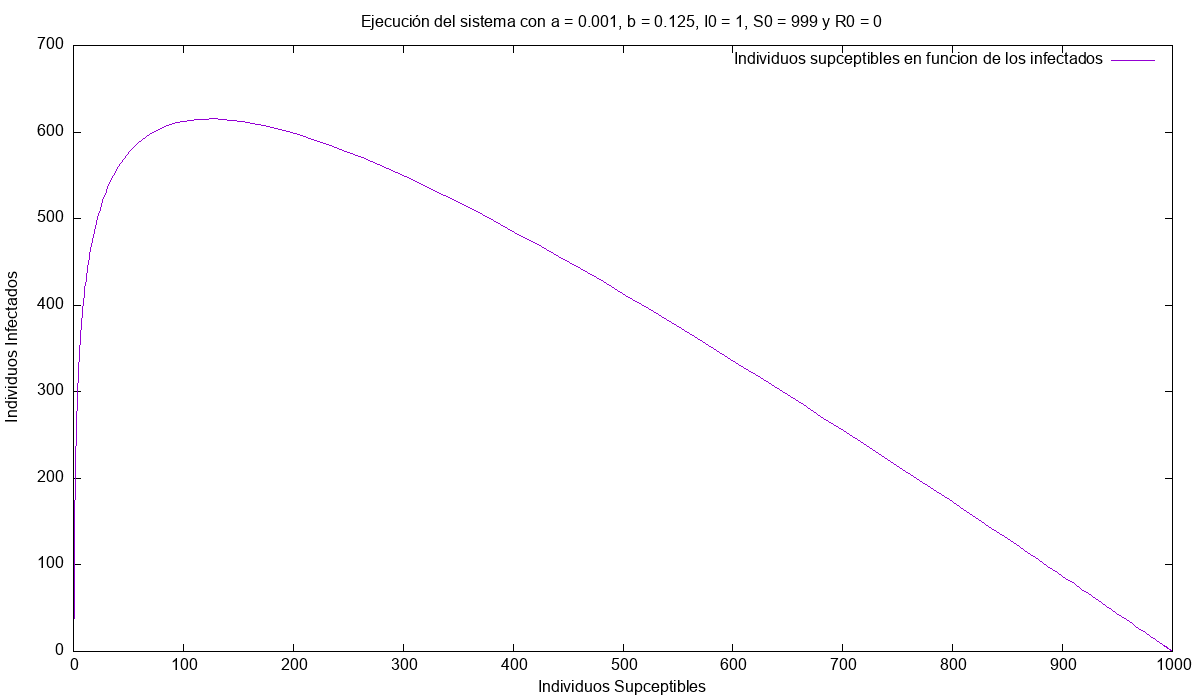
\includegraphics[width=\textwidth]{SIR_planoSI.png}
 		\caption{Individuos supceptibles en funcion de los infectados.}
\end{figure}

Esta gráfica nos muestra como cuando todos los individuos son supceptibles no tenemos ningún individuo infectado, y esta gráfica nos muestra que cuando tenemos el mayor número de infectados es cuando los supceptibles han disminuido drásticamente, pero sin llegar a cero, ya que si no no quedarían individuos por infectar.


\section{Variación de los parámetros del sistema}

En este apartado comprobaremos el significado antes comentado de los parámetros $a$ y $b$. Como he comentado en los apartados anteriores, la $a$ está relacionada con la capacidad de infección y $b$ está relacionada con el tiempo de duración de la enfermedad.

Dentro de este apartado veremos en profundidad como afectan esas variables al sistema.

\subsection{Menor a (disminución de contactos)}

Una reducción del parámetro $a$ supondrá una disminución de los contactos, por lo que en este caso es de esperar que aunque el tamaño de la población es el mismo, aunque al no modificar el parámetro $b$ la duración de la enfermedad es igual, el disminuir los contactos hará que sea más dificil propagar la enfermedad. Para este apartado he reducido a la mitad el valor de $a$:

\begin{figure}[H]
  \centering
      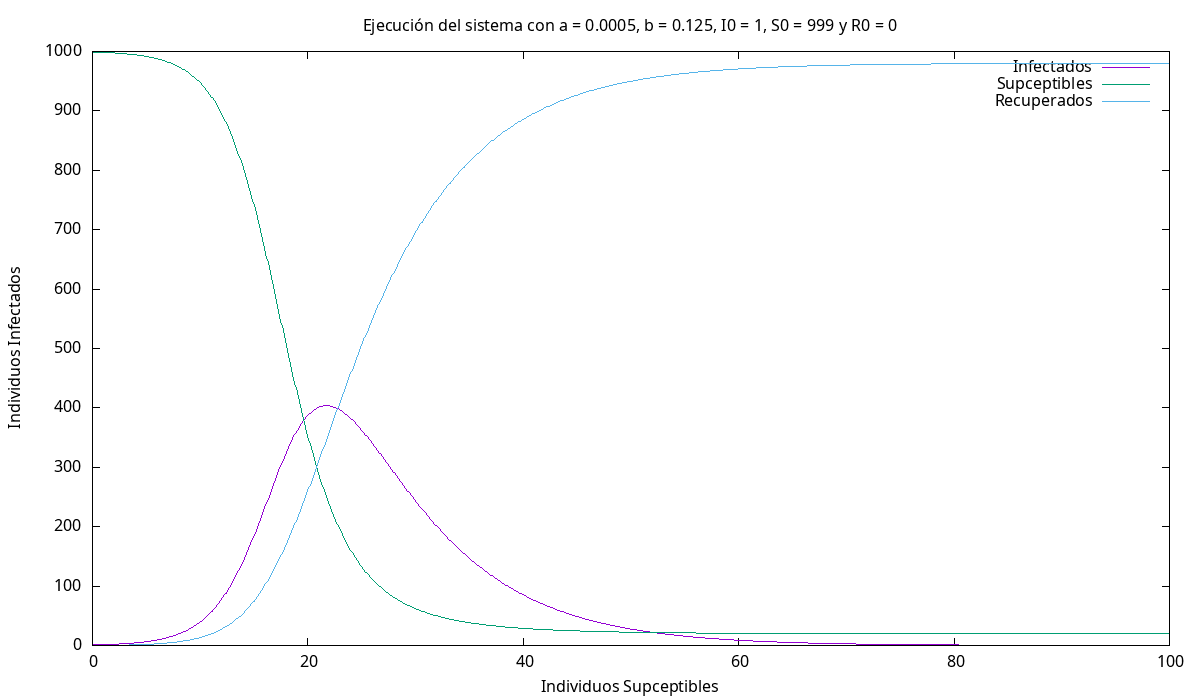
\includegraphics[width=\textwidth]{SIR_menor_a.png}
 		\caption{Simulación con $a = 0.0005$.}
\end{figure}

En este caso vemos como la curva de infectados es mucho más plana que en la simulación original, tal y como esperabamos, se producen menos infecciones e incluso no se llega a infectar a toda la población ya que en el momento que quedan pocos individuos supceptibles la disminución de contactos hace que la enfermedad desaparezca antes de poder seguir contagiando a la poca gente que queda supceptible.

\subsection{Mayor b (mejores tratamientos)}

Una aumento del parámetro $b$ supondrá una disminución de la duración de la enfermedad, por lo que en este caso es de esperar que aunque la capacidad de infección es la misma al no modificar el parámetro $a$, la duración de la enfermedad sea menor al aumentar el valor de $b$. Para este apartado he reducido a la mitad el valor de $b$:

\begin{figure}[H]
	 \centering
	 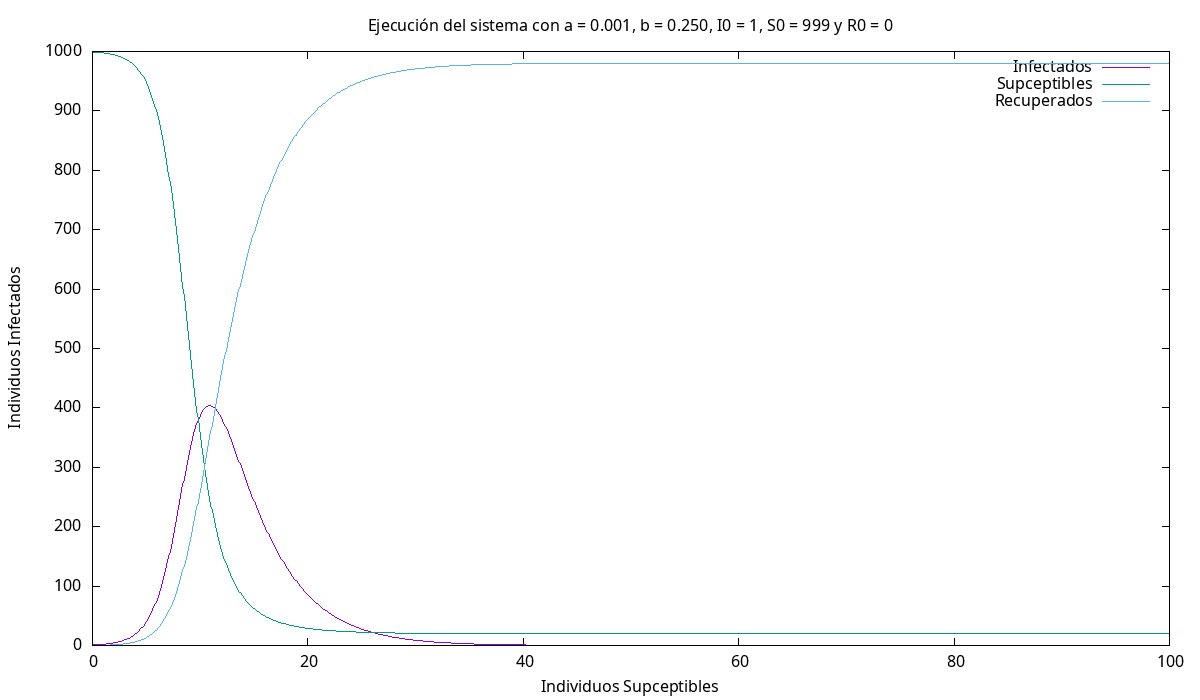
\includegraphics[width=\textwidth]{SIR_mayor_b.png}
		\caption{Simulación con $b = 0.250$.}
\end{figure}

En este apartado ocurre igual que en el apartado anterior, aunque hay una diferencia clave, los infectados ocurren en mucho menor tiempo. Al mantener la infectividad de la enfermedad, pero tener un plazo menor de enfermedad, no se suaviza la curva inicial de infectados, pero si que es más dificil mantenerla como en el apartado inicial, ya que los individuos se recuperan mucho más fácilmente. Por este motivo, aunque no se llega a infectar toda la población debido a que el periodo de enfermedad es más bajo, la curva es mucho más estrecha en tiempo.

\subsection{Aplicar ambos cambios: Menor a (menor capacidad de infección) y mayor b (mejores tratamientos)}

Tras ver los resultados de los apartados anteriores, si aplicamos ambas mejoras a la vez solo cabe suponer que la curva de infectados será mucho más plana. Además de que la capacidad de infección es menor, si la enfermedad se prolonga menos en el tiempo el número de infectados se dilatará en el tiempo, ya que para la enfermedad será mucho más dificil de propagarse.

\begin{figure}[H]
  \centering
      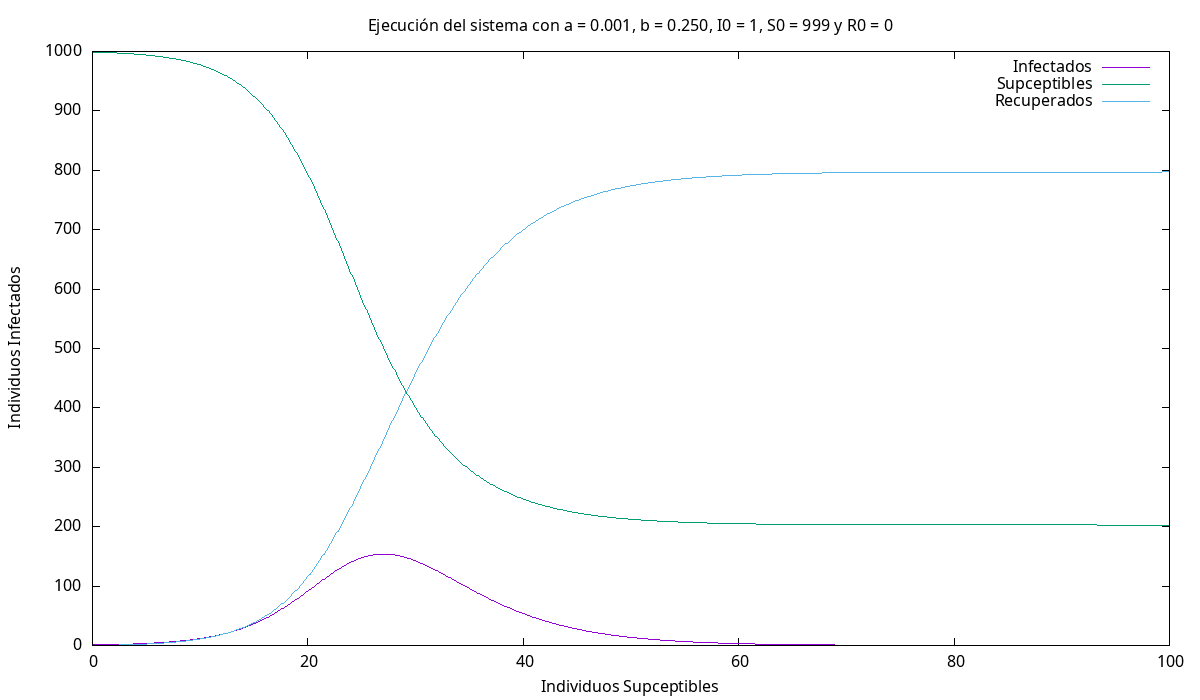
\includegraphics[width=\textwidth]{SIR_menor_a_mayor_b.png}
 		\caption{Simulación con $a = 0.0005$ y $b = 0.250$.}
\end{figure}

Como suponiamos, la enfermedad tarda mucho más en crecer con el tiempo siendo esta ejecución la de menor número infectados y la que más aplanada está dicha curva.


\section{Modificación del número inicial de infectados o inmunes: Inmunidad de grupo}

En apartados anteriores hemos visto como en ocasiones parte de la población supceptible nunca se llegaba a contagiar debido a que la enfermedad desaparecía antes de infectar a parte de la población, sin embargo, ¿que porcentaje de la población es necesario que sea inmune para que pueda existir un grupo supceptible y que desaparezca la enfermedad? En este apartado buscaremos ese porcentaje aumentando progresivamente la cantidad de población recuperada inicial, pero manteniendo el mismo tamaño de población en todos los casos. Tras ejecutar con distintos valores, obtenemos lo siguiente:

\newcounter{recuperados}
\forloop[50]{recuperados}{50}{\value{recuperados} < 901}{
	\begin{figure}[H]
	\centering
			\includegraphics[width=\textwidth]{SIR_inmunidad_\therecuperados.png}
			\caption{Simulación con $R_0 =$ \therecuperados.}
	\end{figure}
}



\section{Comparación entre el método de Euler y el método de Runge-Kutta}


% \begin{thebibliography}{9}
%
%
% \end{thebibliography}

\end{document}
